\documentclass{article}
\usepackage{graphicx}
\usepackage{ctex}
\usepackage{hyperref}
\usepackage{array}
\usepackage{longtable}
\usepackage{hyperref}
\usepackage{verbatim}
\usepackage{geometry}
\usepackage{float}
\usepackage{listings}
\usepackage{algorithm}
\usepackage{minted}
\usepackage{listings}
\usepackage{xcolor}

\lstset
{
    numbers=left, 
    numberstyle=\tiny, 
    keywordstyle=\color{blue!70},
    commentstyle=\color{red!50!green!50!blue!50},
    frame=shadowbox,
    rulesepcolor=\color{red!20!green!20!blue!20},
    escapeinside=``,
    xleftmargin=2em,
    aboveskip=1em,
    framexleftmargin=2em,
    basicstyle=\ttfamily,
    columns=fullflexible,
    linewidth=1\linewidth,
    breaklines=true,
    showstringspaces=false,
    breakatwhitespace=ture,
    escapechar=`
}

\geometry{a4paper,scale=0.8}
\hypersetup{hidelinks,colorlinks=true,allcolors=black,pdfstartview=Fit,breaklinks=true}

\begin{document}

\begin{titlepage}
    \newgeometry{top=6cm}
    \begin{center}
        \bfseries\Huge{软件说明书}\\
        \vspace{0.5cm}
        \bfseries\Large{基于SpringBoot\&Vue的在线考试系统}
        \vspace{5cm}
        \begin{center}\Large\linespread{2}
        \renewcommand\arraystretch{1.6}
        \begin{tabular}{cc}
            \bfseries{单位:} & 计算机学院\\ \cline{2-2}
            \bfseries{班级:} & 2021级计算机科学与技术1班\\ \cline{2-2}
            \bfseries{组长:} & 202105566211 胡翌晨\\ \cline{2-2}
            \bfseries{组员1:} & 202105566219 张家瑞\\ \cline{2-2}
            \bfseries{组员2:} & 202105566202 刁坤明\\ \cline{2-2}
            \bfseries{组员3:} & 202105566213 文鑫\\ \cline{2-2}
            \bfseries{组员4:} & 202105566216 周书法\\ \cline{2-2}
        \end{tabular}
        \end{center}
        \vspace{2cm}
        \Large{湘潭大学\\2024年6月}
    \end{center}
    \thispagestyle{empty}
    \restoregeometry
\end{titlepage}

\newpage
\tableofcontents
\newpage

\section{项目概述}

\subsection{概述}
在线考试系统是一种基于互联网的教育技术工具,旨在为学生、教师或培训机构提供便捷的考试和评估方式。该系统基于SpringBoot+Vue,结合了后端和前端的强大功能,提供了稳定、高效的用户体验。该系统的后端的SpringBoot框架具备快速开发和简化配置的特点,它实现了用户管理、考试管理、试卷管理和成绩管理等核心功能,同时集成了Spring Security来确保用户身份验证和权限管理的安全性。使用Spring Data JPA简化了对数据库的访问和操作,提高了开发效率。前端则采用了Vue.js框架,拥有响应式和组件化的特点,提供了流畅的用户界面和良好的交互体验。它实现了用户登录、考试列表、试卷详情、成绩查询等功能,利用Vue Router实现了页面路由,实现了单页面应用的效果,同时结合了Element UI等UI组件库来美化页面样式,并提供丰富的交互组件。数据交互方面,采用了RESTful API实现前后端的数据交互,实现了前后端分离的架构。前端通过HTTP请求向后端发送数据请求,后端处理请求并返回相应的数据,实现了前后端的数据交互和通信。系统的数据库部分使用关系型数据库来存储用户信息、试卷信息、考试成绩等数据,同时利用Spring Data JPA简化了对数据库的操作,提高了数据访问的效率和便捷性。

\subsection{代码托管}
\href{https://github.com/Jarrett-Zhang/Information-System-Development}{https://github.com/Jarrett-Zhang/Information-System-Development}

\subsection{小组分工}
\begin{center}
\begin{tabular}{c|c}
胡翌晨 & 前/后端代码实现\\
张家瑞 & 需求分析、系统设计、项目测试\\
刁坤明 & SpringBoot开发\\
文鑫 & Vue开发\\
周书法 & UI/UX设计、项目测试\\
\end{tabular}
\end{center}

\subsection{工作进度}
\begin{center}
\begin{tabular}{c|c}
2024.6.18 & 确认选题\\
2024.6.19 $\sim$ 2024.6.20 & 需求分析\\
2024.6.21 $\sim$ 2024.6.23 & 系统设计\\
2024.6.19 $\sim$ 2024.6.23 & 编写项目计划书\\
2024.6.24 $\sim$ 2024.6.29 & 代码编写\\
2024.6.30 $\sim$ 2024.7.1 & 项目测试\\
2024.6.30 $\sim$ 2024.7.1 & 编写项目说明书
\end{tabular}
\end{center}


\section{需求分析}

\subsection{用例图}
\begin{figure}[H]
    \centering
    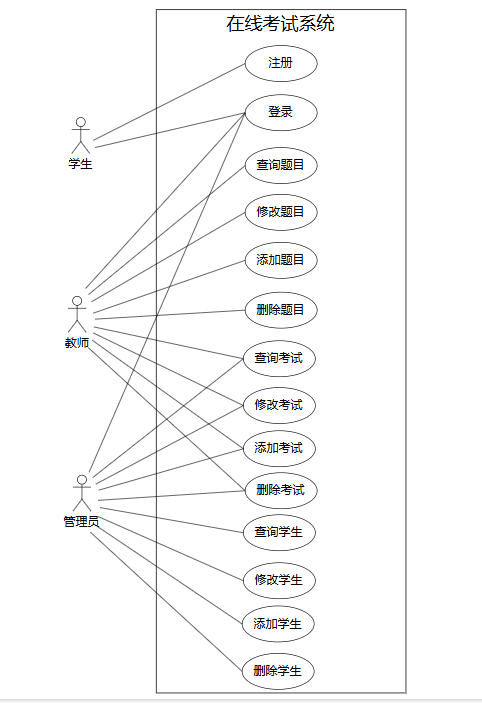
\includegraphics[width=0.85\linewidth]{use-case diagram.png}
\end{figure}

\subsection{用例模型}
\begin{centering}
\begin{longtable}{|c|m{11cm}<{\centering}|} \hline
\textbf{用例编号与名称} & UC001:登录 \\ \hline
\textbf{范围} & 在线考试系统 \\ \hline
\textbf{级别} & 用户目标 \\ \hline
\textbf{主要参与者} & 所有用户 \\ \hline
\textbf{涉众及其关注点} & 用户希望能够通过输入正确的凭据进入系统 \\ \hline
\textbf{前置条件} & 数据库和后端服务器正常运行;用户处于登录界面 \\ \hline
\textbf{成功保证} & 用户输入正确的账号和密码后点击登录按钮 \\ \hline
\textbf{主成功场景} & 用户输入正确的账号和密码,点击登录按钮后成功进入系统 \\ \hline
\textbf{扩展} & 如果用户输入的账号或密码不正确,系统应提示用户重新输入 \\ \hline
\textbf{特殊需求} & 用户登录后,系统需要将用户信息保存为全局变量以便后续使用 \\ \hline
\textbf{技术与数据变元素} & 输入账号和密码;点击登录按钮 \\ \hline
\textbf{发生频率} & 用户每次访问系统时需进行登录 \\ \hline
\textbf{杂项} & 不同权限的用户登录后会进入不同的系统模块,确保各模块之间的隔离 \\ \hline
\multicolumn{1}{c@{}}{} & \multicolumn{1}{c@{}}{} \\ \hline
\textbf{用例编号与名称} & UC002:注册 \\ \hline
\textbf{范围} & 在线考试系统 \\ \hline
\textbf{级别} & 用户目标 \\ \hline
\textbf{主要参与者} & 学生 \\ \hline
\textbf{涉众及其关注点} & 学生希望能够注册账号参加在线考试,管理员关注注册流程的管理和信息安全 \\ \hline
\textbf{前置条件} & 用户打开注册页面且系统处于正常运行状态 \\ \hline
\textbf{成功保证} & 系统能够安全地存储用户提供的注册信息 \\ \hline
\textbf{主成功场景} & 用户填写正确的注册信息并成功提交后,系统将信息存入数据库并提示注册成功 \\ \hline
\textbf{扩展} & 如果用户输入的信息格式不正确或用户名已存在,系统应给予相应提示并要求修正 \\ \hline
\textbf{特殊需求} & 用户密码需加密存储,用户名和邮箱需唯一性检查 \\ \hline
\textbf{技术与数据变元素} & 输入包括用户名、密码、邮箱等信息,输出为注册成功/失败的消息 \\ \hline
\textbf{发生频率} & 根据学生注册需求和管理员审批频率而定 \\ \hline
\textbf{杂项} & 注册页面设计需考虑用户体验和信息安全的平衡 \\ \hline
\multicolumn{1}{c@{}}{} & \multicolumn{1}{c@{}}{} \\ \hline
\textbf{用例编号与名称} & UC003:查询学生 \\ \hline
\textbf{范围} & 在线考试系统 \\ \hline
\textbf{级别} & 用户目标 \\ \hline
\textbf{主要参与者} & 管理员 \\ \hline
\textbf{涉众及其关注点} & 管理员希望能够快速准确地查找特定学生的信息 \\ \hline
\textbf{前置条件} & 管理员已登录系统并进入学生管理界面 \\ \hline
\textbf{成功保证} & 系统能够根据管理员提供的查询条件,有效地检索并显示符合条件的学生信息 \\ \hline
\textbf{主成功场景} & 管理员输入学生的姓名或学号进行查询,系统显示匹配的学生信息列表 \\ \hline
\textbf{扩展} & 如果查询结果为空或查询条件格式错误,系统应提供相应的提示信息 \\ \hline
\textbf{特殊需求} & 查询操作应考虑数据库索引的优化,以提高查询效率 \\ \hline
\textbf{技术与数据变元素} & 输入查询条件(学生姓名或学号),输出符合条件的学生信息列表 \\ \hline
\textbf{发生频率} & 管理员根据学校管理和教学安排的需要进行学生信息查询 \\ \hline
\textbf{杂项} & 需要确保查询操作的权限控制,只有授权的管理员能够访问学生信息 \\ \hline
\multicolumn{1}{c@{}}{} & \multicolumn{1}{c@{}}{} \\ \hline
\textbf{用例编号与名称} & UC004:添加学生 \\ \hline
\textbf{范围} & 在线考试系统 \\ \hline
\textbf{级别} & 用户目标 \\ \hline
\textbf{主要参与者} & 管理员 \\ \hline
\textbf{涉众及其关注点} & 管理员希望能够向系统中添加新的学生信息 \\ \hline
\textbf{前置条件} & 管理员已登录系统并进入学生管理界面 \\ \hline
\textbf{成功保证} & 系统能够安全、准确地存储新添加学生的信息至数据库 \\ \hline
\textbf{主成功场景} & 管理员输入新学生的必要信息(如姓名、学号、班级等),系统保存信息并显示添加成功的消息 \\ \hline
\textbf{扩展} & 如果输入的学生信息格式不正确或数据库保存失败,系统应提示管理员重新输入或联系技术支持 \\ \hline
\textbf{特殊需求} & 添加操作需要确保学生信息的唯一性和完整性,避免重复添加或信息缺失 \\ \hline
\textbf{技术与数据变元素} & 输入新学生的信息(如姓名、学号、班级等),点击添加按钮 \\ \hline
\textbf{发生频率} & 管理员根据学校的入学或信息更新需求定期进行学生信息的添加操作 \\ \hline
\textbf{杂项} & 管理员应具备足够的权限来执行学生信息的添加操作,系统界面应设计友好、易用以便管理员操作 \\ \hline
\multicolumn{1}{c@{}}{} & \multicolumn{1}{c@{}}{} \\ \hline
\textbf{用例编号与名称} & UC005:修改学生 \\ \hline
\textbf{范围} & 在线考试系统 \\ \hline
\textbf{级别} & 用户目标 \\ \hline
\textbf{主要参与者} & 管理员 \\ \hline
\textbf{涉众及其关注点} & 管理员希望能够修改特定学生的个人信息 \\ \hline
\textbf{前置条件} & 管理员已登录系统并进入学生管理界面 \\ \hline
\textbf{成功保证} & 系统能够安全、准确地修改学生的信息并更新至数据库 \\ \hline
\textbf{主成功场景} & 管理员选定特定学生,修改其个人信息(如姓名、联系方式等),保存修改后的信息 \\ \hline
\textbf{扩展} & 如果管理员输入的修改信息格式不正确或数据库更新失败,系统应提示管理员重新尝试或联系技术支持 \\ \hline
\textbf{特殊需求} & 修改操作需要记录修改历史以便追溯,确保数据的完整性和安全性 \\ \hline
\textbf{技术与数据变元素} & 输入修改后的学生信息(如姓名、联系方式等),点击保存按钮 \\ \hline
\textbf{发生频率} & 根据学生信息变动和管理员操作需求而定,通常在学生信息变更时进行 \\ \hline
\textbf{杂项} & 管理员应有足够的权限来执行学生信息的修改操作,同时操作界面应简洁直观以便管理员操作 \\ \hline
\multicolumn{1}{c@{}}{} & \multicolumn{1}{c@{}}{} \\ \hline
\textbf{用例编号与名称} & UC006:删除学生 \\ \hline
\textbf{范围} & 在线考试系统 \\ \hline
\textbf{级别} & 用户目标 \\ \hline
\textbf{主要参与者} & 管理员 \\ \hline
\textbf{涉众及其关注点} & 管理员希望能够从系统中删除特定的学生信息 \\ \hline
\textbf{前置条件} & 管理员已登录系统并进入学生管理界面 \\ \hline
\textbf{成功保证} & 系统能够安全、有效地从数据库中删除指定学生的信息 \\ \hline
\textbf{主成功场景} & 管理员选择特定学生,确认删除操作后,系统从数据库中删除该学生的信息并显示删除成功的消息 \\ \hline
\textbf{扩展} & 如果管理员选择的学生信息有误或数据库删除操作失败,系统应提示管理员重新确认或联系技术支持 \\ \hline
\textbf{特殊需求} & 删除操作需谨慎执行,系统可能需要记录删除操作的日志以便追溯和恢复 \\ \hline
\textbf{技术与数据变元素} & 选择特定学生的信息进行删除确认操作 \\ \hline
\textbf{发生频率} & 管理员根据学校的管理需要和学生信息变动情况定期执行学生信息的删除操作 \\ \hline
\textbf{杂项} & 管理员应具备足够的权限来执行学生信息的删除操作,系统界面应设计友好、操作流程清晰以便管理员操作 \\ \hline
\multicolumn{1}{c@{}}{} & \multicolumn{1}{c@{}}{} \\ \hline
\textbf{用例编号与名称} & UC007:查询题目 \\ \hline
\textbf{范围} & 在线考试系统 \\ \hline
\textbf{级别} & 用户目标 \\ \hline
\textbf{主要参与者} & 教师 \\ \hline
\textbf{涉众及其关注点} & 教师希望能够快速准确地查找特定的题目信息 \\ \hline
\textbf{前置条件} & 教师已登录系统并进入题库管理界面 \\ \hline
\textbf{成功保证} & 系统能够根据教师提供的查询条件,有效地检索并显示符合条件的题目信息 \\ \hline
\textbf{主成功场景} & 教师输入题目关键词或题目编号进行查询,系统显示匹配的题目信息列表 \\ \hline
\textbf{扩展} & 如果查询结果为空或查询条件格式不正确,系统应提示教师重新输入 \\ \hline
\textbf{特殊需求} & 查询操作需要考虑题目库的索引优化,以提高查询效率 \\ \hline
\textbf{技术与数据变元素} & 输入查询条件(题目关键词或题目编号),输出符合条件的题目信息列表 \\ \hline
\textbf{发生频率} & 教师根据课程教学需求和题目变动情况进行题目信息查询 \\ \hline
\textbf{杂项} & 需要确保查询操作的权限控制,只有授权的教师能够访问题目信息 \\ \hline
\multicolumn{1}{c@{}}{} & \multicolumn{1}{c@{}}{} \\ \hline
\textbf{用例编号与名称} & UC008:添加题目 \\ \hline
\textbf{范围} & 在线考试系统 \\ \hline
\textbf{级别} & 用户目标 \\ \hline
\textbf{主要参与者} & 教师 \\ \hline
\textbf{涉众及其关注点} & 教师希望能够向系统中添加新的题目信息 \\ \hline
\textbf{前置条件} & 教师已登录系统并进入题库管理界面 \\ \hline
\textbf{成功保证} & 系统能够安全、准确地存储新添加的题目信息至题库 \\ \hline
\textbf{主成功场景} & 教师输入新题目的各项信息(如题目内容、选项、答案等),系统保存信息并显示添加成功的消息 \\ \hline
\textbf{扩展} & 如果输入的题目信息格式不正确或保存失败,系统应提示教师重新输入或联系技术支持 \\ \hline
\textbf{特殊需求} & 添加操作需要确保题目信息的唯一性和完整性 \\ \hline
\textbf{技术与数据变元素} & 输入新题目的信息(如题目内容、选项、答案等),点击添加按钮 \\ \hline
\textbf{发生频率} & 教师根据课程教学需求和题目变动情况定期进行题目信息的添加操作 \\ \hline
\textbf{杂项} & 系统应设计友好、易用的界面以便教师操作,同时保证操作流程清晰 \\ \hline
\multicolumn{1}{c@{}}{} & \multicolumn{1}{c@{}}{} \\ \hline
\textbf{用例编号与名称} & UC009:修改题目 \\ \hline
\textbf{范围} & 在线考试系统 \\ \hline
\textbf{级别} & 用户目标 \\ \hline
\textbf{主要参与者} & 教师 \\ \hline
\textbf{涉众及其关注点} & 教师希望能够修改题库中特定题目的信息 \\ \hline
\textbf{前置条件} & 教师已登录系统并进入题库管理界面 \\ \hline
\textbf{成功保证} & 系统能够安全、准确地更新题库中特定题目的信息 \\ \hline
\textbf{主成功场景} & 教师选择特定题目,修改其内容(如题目内容、选项、答案等),保存修改后的信息 \\ \hline
\textbf{扩展} & 如果教师选择的题目信息有误或更新失败,系统应提示教师重新确认或联系技术支持 \\ \hline
\textbf{特殊需求} & 修改操作需要记录修改历史以便追溯,确保数据的完整性和安全性 \\ \hline
\textbf{技术与数据变元素} & 选择特定题目的信息进行修改操作 \\ \hline
\textbf{发生频率} & 根据教师的教学需求和题目信息变动情况进行题目信息的修改操作 \\ \hline
\textbf{杂项} & 系统应确保操作界面清晰,避免误操作,同时提供友好的用户反馈 \\ \hline
\multicolumn{1}{c@{}}{} & \multicolumn{1}{c@{}}{} \\ \hline
\textbf{用例编号与名称} & UC010:删除题目 \\ \hline
\textbf{范围} & 在线考试系统 \\ \hline
\textbf{级别} & 用户目标 \\ \hline
\textbf{主要参与者} & 教师 \\ \hline
\textbf{涉众及其关注点} & 教师希望能够从题库中删除特定的题目 \\ \hline
\textbf{前置条件} & 教师已登录系统并进入题库管理界面 \\ \hline
\textbf{成功保证} & 系统能够安全、有效地从数据库中删除指定题目的信息 \\ \hline
\textbf{主成功场景} & 教师选择特定题目,确认删除操作后,系统从数据库中删除该题目并显示删除成功的消息 \\ \hline
\textbf{扩展} & 如果教师选择的题目信息有误或数据库删除操作失败,系统应提示教师重新确认或联系技术支持 \\ \hline
\textbf{特殊需求} & 删除操作需谨慎执行,系统可能需要记录删除操作的日志以便追溯和恢复 \\ \hline
\textbf{技术与数据变元素} & 选择特定题目的信息进行删除确认操作 \\ \hline
\textbf{发生频率} & 教师根据课程教学需求和题目变动情况定期进行题目信息的删除操作 \\ \hline
\textbf{杂项} & 系统应确保操作界面简洁明了,避免误操作,同时提供清晰的用户操作指导 \\ \hline
\multicolumn{1}{c@{}}{} & \multicolumn{1}{c@{}}{} \\ \hline
\textbf{用例编号与名称} & UC011:查询考试 \\ \hline
\textbf{范围} & 在线考试系统 \\ \hline
\textbf{级别} & 用户目标 \\ \hline
\textbf{主要参与者} & 教师、管理员 \\ \hline
\textbf{涉众及其关注点} & 教师和管理员希望能够快速准确地查找特定的考试信息 \\ \hline
\textbf{前置条件} & 用户已登录系统并进入考试管理界面 \\ \hline
\textbf{成功保证} & 系统能够根据用户提供的查询条件,有效地检索并显示符合条件的考试信息 \\ \hline
\textbf{主成功场景} & 用户输入考试名称或考试编号进行查询,系统显示匹配的考试信息列表 \\ \hline
\textbf{扩展} & 如果查询结果为空或查询条件格式不正确,系统应提示用户重新输入 \\ \hline
\textbf{特殊需求} & 查询操作需要考虑考试信息的索引优化,以提高查询效率 \\ \hline
\textbf{技术与数据变元素} & 输入查询条件(考试名称或考试编号),输出符合条件的考试信息列表 \\ \hline
\textbf{发生频率} & 教师和管理员根据学校的管理和教学安排需求进行考试信息的查询 \\ \hline
\textbf{杂项} & 系统应设计灵活的查询界面和权限控制,确保只有授权的用户能够访问考试信息 \\ \hline
\multicolumn{1}{c@{}}{} & \multicolumn{1}{c@{}}{} \\ \hline
\textbf{用例编号与名称} & UC012:添加考试 \\ \hline
\textbf{范围} & 在线考试系统 \\ \hline
\textbf{级别} & 用户目标 \\ \hline
\textbf{主要参与者} & 教师、管理员 \\ \hline
\textbf{涉众及其关注点} & 教师和管理员希望能够向系统中添加新的考试信息 \\ \hline
\textbf{前置条件} & 用户已登录系统并进入考试管理界面 \\ \hline
\textbf{成功保证} & 系统能够安全、准确地存储新添加的考试信息至数据库 \\ \hline
\textbf{主成功场景} & 用户输入新考试的各项信息(如考试名称、时间、地点等),系统保存信息并显示添加成功的消息 \\ \hline
\textbf{扩展} & 如果输入的考试信息格式不正确或保存失败,系统应提示用户重新输入或联系技术支持 \\ \hline
\textbf{特殊需求} & 添加操作需要确保考试信息的唯一性和完整性 \\ \hline
\textbf{技术与数据变元素} & 输入新考试的信息(如考试名称、时间、地点等),点击添加按钮 \\ \hline
\textbf{发生频率} & 教师和管理员根据学校的考试安排和管理需求定期进行考试信息的添加操作 \\ \hline
\textbf{杂项} & 系统应提供简单易用的操作界面,确保用户能够轻松完成添加操作 \\ \hline
\multicolumn{1}{c@{}}{} & \multicolumn{1}{c@{}}{} \\ \hline
\textbf{用例编号与名称} & UC013:修改考试 \\ \hline
\textbf{范围} & 在线考试系统 \\ \hline
\textbf{级别} & 用户目标 \\ \hline
\textbf{主要参与者} & 教师、管理员 \\ \hline
\textbf{涉众及其关注点} & 教师和管理员希望能够修改已有的考试信息 \\ \hline
\textbf{前置条件} & 用户已登录系统并进入考试管理界面 \\ \hline
\textbf{成功保证} & 系统能够安全、准确地更新数据库中特定考试的信息 \\ \hline
\textbf{主成功场景} & 用户选择特定考试,修改其相关信息(如考试名称、时间、地点等),保存修改后的信息 \\ \hline
\textbf{扩展} & 如果用户选择的考试信息有误或更新失败,系统应提示用户重新确认或联系技术支持 \\ \hline
\textbf{特殊需求} & 修改操作需要记录修改历史以便追溯,确保数据的完整性和安全性 \\ \hline
\textbf{技术与数据变元素} & 选择特定考试的信息进行修改操作 \\ \hline
\textbf{发生频率} & 根据学校的考试安排和管理需求定期进行考试信息的修改操作 \\ \hline
\textbf{杂项} & 系统应提供清晰、直观的操作界面,确保用户能够轻松完成修改操作 \\ \hline
\multicolumn{1}{c@{}}{} & \multicolumn{1}{c@{}}{} \\ \hline
\textbf{用例编号与名称} & UC014:删除考试 \\ \hline
\textbf{范围} & 在线考试系统 \\ \hline
\textbf{级别} & 用户目标 \\ \hline
\textbf{主要参与者} & 教师、管理员 \\ \hline
\textbf{涉众及其关注点} & 教师和管理员希望能够从系统中删除特定的考试信息 \\ \hline
\textbf{前置条件} & 用户已登录系统并进入考试管理界面 \\ \hline
\textbf{成功保证} & 系统能够安全、有效地从数据库中删除指定考试的信息 \\ \hline
\textbf{主成功场景} & 用户选择特定考试,确认删除操作后,系统从数据库中删除该考试并显示删除成功的消息 \\ \hline
\textbf{扩展} & 如果用户选择的考试信息有误或数据库删除操作失败,系统应提示用户重新确认或联系技术支持 \\ \hline
\textbf{特殊需求} & 删除操作需谨慎执行,系统可能需要记录删除操作的日志以便追溯和恢复 \\ \hline
\textbf{技术与数据变元素} & 选择特定考试的信息进行删除确认操作 \\ \hline
\textbf{发生频率} & 根据学校的考试安排和管理需求定期进行考试信息的删除操作 \\ \hline
\textbf{杂项} & 系统应提供直观、安全的操作界面,避免误操作,同时提供清晰的用户反馈 \\ \hline
\end{longtable}
\end{centering}

\subsection{补充性规格说明}
\begin{itemize}
    \item \textbf{安全性要求}:用户密码必须加密存储,所有敏感数据传输必须通过HTTPS加密
    \item \textbf{性能要求}:系统应能够支持大量同时在线用户,并保持良好的响应速度,查询和操作题目、考试信息的平均响应时间不超过1秒
    \item \textbf{可靠性要求}:系统应具备高可用性,故障恢复时间应不超过30分钟,确保在99\%的时间内可供用户访问和操作
    \item \textbf{界面设计要求}:系统应具备直观友好的用户界面,保证用户能够快速上手使用,操作流程简洁明了
    \item \textbf{数据库要求}:题目、考试等信息的数据库应具备良好的结构化设计,确保数据存储的一致性和完整性
    \item \textbf{扩展性要求}:系统应支持模块化设计和可扩展性架构,便于未来根据需求扩展新功能或集成新模块
\end{itemize}

\subsection{词汇表}
\begin{itemize}
    \item \textbf{学生}:使用在线考试系统进行考试和学习的注册用户
    \item \textbf{教师}:负责管理和监督学生考试以及题库内容的用户
    \item \textbf{管理员}:系统的管理者,负责整体系统的配置、维护和用户管理
    \item \textbf{题目}:用于在线考试的问题或任务
    \item \textbf{考试}:一组题目的集合
    \item \textbf{界面}:系统和用户之间进行交互的视觉和操作界面
\end{itemize}

\subsection{设想}
本系统是一个基于Spring Boot和Vue.js开发的在线考试系统,旨在为学校、培训机构或企业提供一个灵活、高效的考试管理平台

\subsection{业务规则}
\begin{itemize}
    \item 在系统中通过用户登陆的角色不同,进入不同的用户管理界面
    \item 不同的用户可以在相应的页面查询和修改信息
    \item 用户权限不同,对数据的操作权限也不同
\end{itemize}

\section{系统设计}

\subsection{操作契约}
\begin{itemize}
    \item \textbf{操作}:登录\\
        \textbf{参数}:账号(String)、密码(String)\\
        \textbf{交叉引用}:用例"登录"\\
        \textbf{前置条件}:无\\
        \textbf{后置条件}:
        \begin{itemize}
            \item 如果用户名和密码匹配且通过验证,则用户成功登录系统
            \item 如果验证失败(用户名不存在或密码不正确),系统将给出相应的错误提示
        \end{itemize}
    \item \textbf{操作}:查询\\
        \textbf{参数}:ID(int)\\
        \textbf{交叉引用}:用例"查询学生/题目/考试"\\
        \textbf{前置条件}:所查ID必须存在于系统中\\
        \textbf{后置条件}:
        \begin{itemize}
            \item 系统根据ID查询并返回对应信息
            \item 如果找不到该ID对应的数据,则返回空结果或相应的提示信息
        \end{itemize}
    \item \textbf{操作}:添加\\
        \textbf{参数}:添加项目信息\\
        \textbf{交叉引用}:用例"添加学生/题目/考试"\\
        \textbf{前置条件}:无\\
        \textbf{后置条件}:
        \begin{itemize}
            \item 在数据库中成功创建新的项目,并保存其信息
            \item 如果操作失败,系统将给出相应的错误提示
        \end{itemize}
\end{itemize}

\subsection{系统时序图}
\begin{comment}
sequenceDiagram
User->>View:启动
View->>Controller:启动
Controller-->>View:返回界面数据
View-->>User:显示UI
User->>View:登录
View->>Controller:输入账号密码
Controller->>Service:HTTP请求
Service->>DataBase:SQL操作
DataBase-->>Service:返回用户数据
Service-->>Controller:返回用户数据
Controller-->>View:判断用户权级
View-->>User:进入系统
User->>View:用户操作
View->>Controller:查询
Controller->>Service:HTTP请求
Service->>DataBase:SQL操作
DataBase-->>Service:返回数据
Service-->>Controller:返回数据
Controller-->>View:返回数据
View->>Controller:修改
Controller->>Service:HTTP请求
Service->>DataBase:SQL操作
DataBase-->>Service:返回影响
Service-->>Controller:返回影响
Controller-->>View:判断是否成功
\end{comment}
\begin{figure}[H]
    \centering
    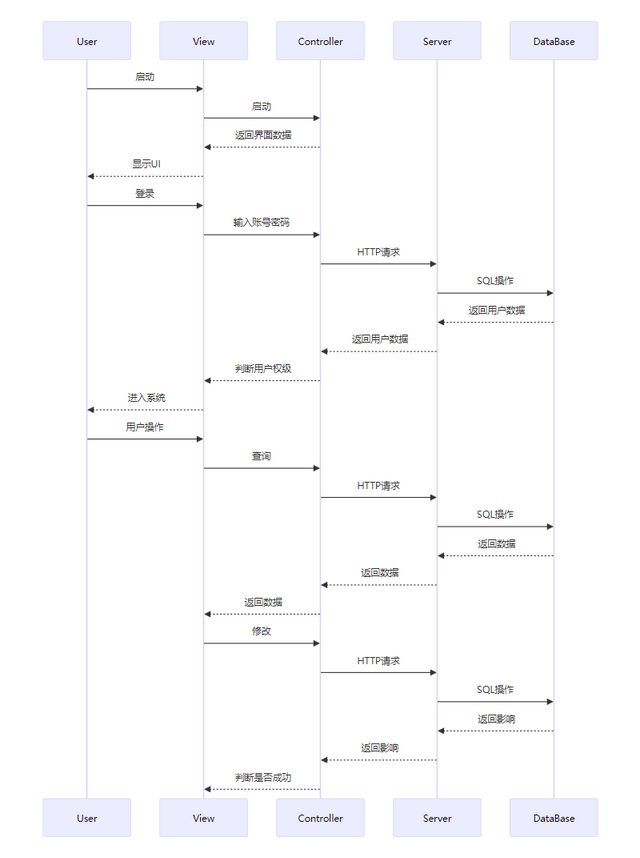
\includegraphics[width=0.95\linewidth]{sequence diagram.png}
\end{figure}

\subsection{包图}
\begin{figure}[H]
    \centering
    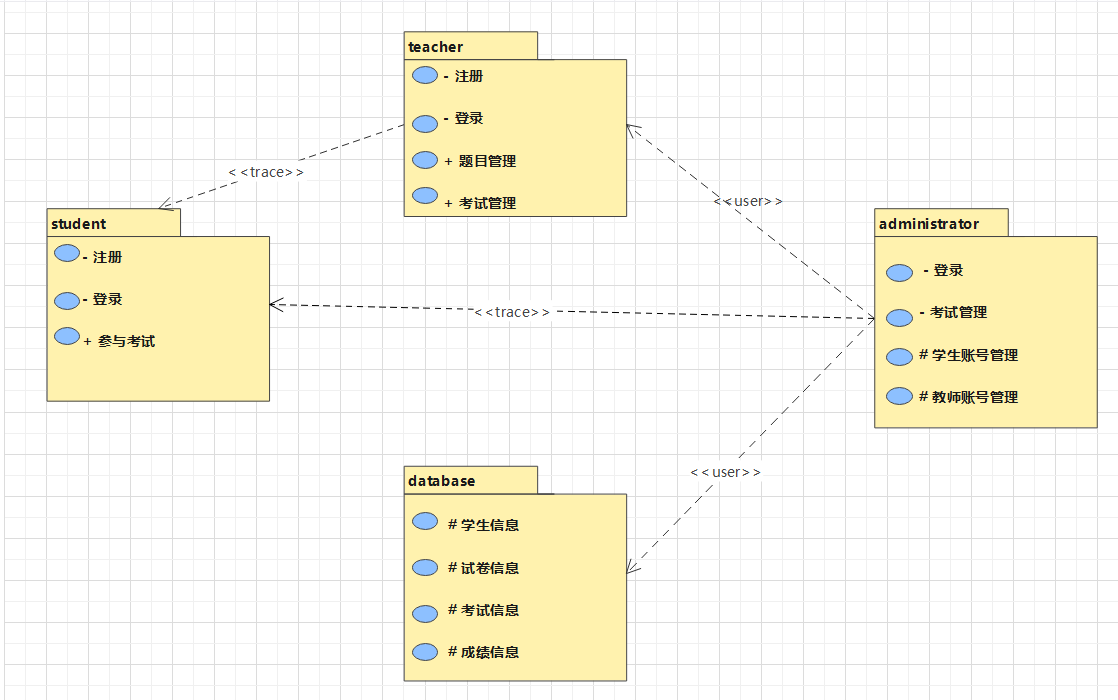
\includegraphics[width=0.8\linewidth]{package diagram.png}
\end{figure}

\subsection{类图}
\begin{figure}[H]
    \centering
    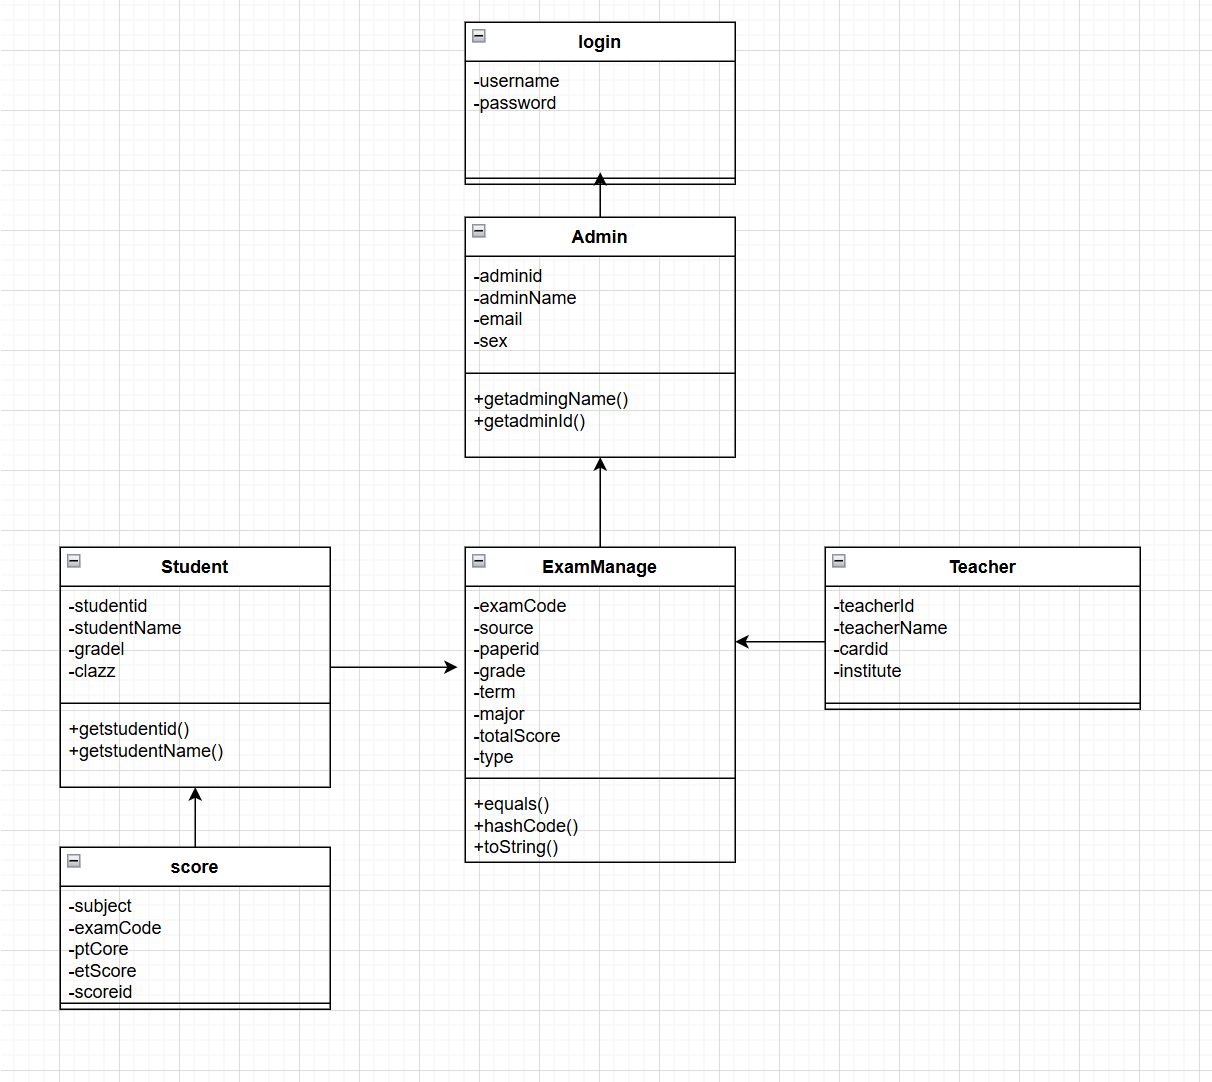
\includegraphics[width=0.8\linewidth]{class diagram.png}
\end{figure}

\subsection{逻辑分层}
\begin{enumerate}
    \item \textbf{View 视图层} \newline
    作用:
        \begin{itemize}
        \item 用户界面的展示和交互
        \item 接收用户的输入操作
        \item 将用户操作传递给控制器处理
        \end{itemize}
    特征:
        \begin{itemize}
        \item HTML、Vue.js等前端技术。
        \item 负责呈现数据和收集用户输入。
        \item 不包含业务逻辑,专注于界面和用户交互。
        \end{itemize}
    \item \textbf{Controller 控制器层} \newline
    作用:
        \begin{itemize}
        \item 处理用户的请求和操作。
        \item 调度和协调系统中的其他组件。
        \item 通常负责路由和请求转发。
        \end{itemize}
    特征:
        \begin{itemize}
        \item Spring、Servlet等框架中的控制器。
        \item 接收来自视图层的请求并调用相应的服务层处理业务逻辑。
        \item 处理输入验证和参数校验,确保传递给服务层的数据有效性。
        \end{itemize}
    \item \textbf{Service 服务层} \newline
    作用:
        \begin{itemize}
        \item 执行业务逻辑和数据处理。
        \item 作为控制器和数据访问层(DAO层)之间的中介。
        \item 可以跨多个控制器共享。
        \end{itemize}
    特征:
        \begin{itemize}
        \item Java类或者Spring的@Service注解类。
        \item 包含业务规则的实现,如数据处理、转换、验证等。
        \item 不直接与用户界面交互,而是接受控制器层传递的请求并返回处理结果。
        \end{itemize}
    \item \textbf{DataBase 数据访问层} \newline
    作用:
        \begin{itemize}
        \item 负责与数据库的交互。
        \item 执行数据的CRUD操作(创建、读取、更新、删除)。
        \item 提供持久化机制,确保数据的安全性和一致性。
        \end{itemize}
    特征:
        \begin{itemize}
        \item DAO(Data Access Object)接口或者实现类。
        \item 使用JDBC、Hibernate、Spring Data等技术实现与数据库的通信。
        \item 负责处理数据库连接、事务管理、数据检索和更新等操作。
        \end{itemize}
\end{enumerate}
\subsection{数据库设计}
\begin{figure}[H]
    \centering
    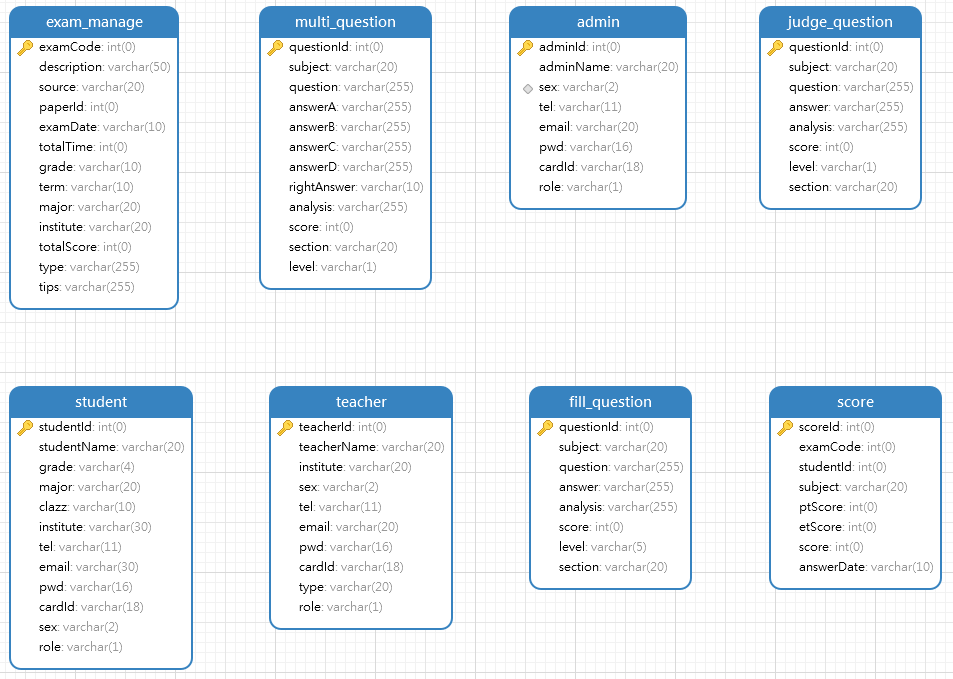
\includegraphics[width=\linewidth]{database design.png}
\end{figure}


\section{代码实现}

\subsection{核心代码示例:登录}

前端:
\lstset{language=java}
\begin{lstlisting}
login() {
  console.log("登录操作执行-------"); // 打印登录操作执行信息

  // 发送登录请求
  this.$axios({
    url: `http://localhost:8080/login/`,
    method: 'post',
    data: {
      ...this.formLabelAlign  // 使用表单数据作为请求体
    }
  }).then(res => {  // 请求成功的回调函数
    let resData = res.data.data;  // 获取响应数据

    // 根据用户角色进行处理
    if (resData != null) {
      switch (resData.role) {
        case "0":  // 管理员
          this.$cookies.set("cname", resData.adminName);  // 设置管理员姓名
          this.$cookies.set("cid", resData.adminId);  // 设置管理员ID
          this.$cookies.set("role", 0);  // 设置角色为管理员
          this.$router.push({ path: '/index' });  // 跳转到首页
          break;
        case "1":  // 教师
          this.$cookies.set("cname", resData.teacherName);  // 设置教师姓名
          this.$cookies.set("cid", resData.teacherId);  // 设置教师ID
          this.$cookies.set("role", 1);  // 设置角色为教师
          this.$router.push({ path: '/index' });  // 跳转到教师用户页面
          break;
        case "2":  // 学生
          this.$cookies.set("cname", resData.studentName);  // 设置学生姓名
          this.$cookies.set("cid", resData.studentId);  // 设置学生ID
          this.$router.push({ path: '/student' });  // 跳转到学生页面
          break;
      }
    }

    // 处理登录失败情况
    if (resData == null) {
      this.$message({
        showClose: true,
        type: 'error',
        message: '用户名或者密码错误'
      });
    }
  });
}

\end{lstlisting}

后端:

\begin{lstlisting}
@Mapper
public interface LoginMapper {

    // 查询管理员登录信息
    @Select("select adminId, adminName, sex, tel, email, cardId, role " +
            "from admin where adminId = #{username} and pwd = #{password}")
    public Admin adminLogin(Integer username, String password);

    // 查询教师登录信息
    @Select("select teacherId, teacherName, institute, sex, tel, email, cardId, " +
            "type, role from teacher where teacherId = #{username} and pwd = #{password}")
    public Teacher teacherLogin(Integer username, String password);

    // 查询学生登录信息
    @Select("select studentId, studentName, grade, major, clazz, institute, tel, " +
            "email, cardId, sex, role from student where studentId = #{username} and pwd = #{password}")
    public Student studentLogin(Integer username, String password);
}

\end{lstlisting}

\subsection{核心代码示例:试卷管理}

\begin{lstlisting}
@Mapper
public interface ExamManageMapper {

    // 查询所有考试信息,并返回列表
    @Select("select * from exam_manage")
    List<ExamManage> findAll1();

    // 分页查询所有考试信息
    @Select("select * from exam_manage")
    IPage<ExamManage> findAll(Page page);

    // 根据考试代码查询考试信息
    @Select("select * from exam_manage where examCode = #{examCode}")
    ExamManage findById(Integer examCode);

    // 根据考试代码删除考试信息
    @Delete("delete from exam_manage where examCode = #{examCode}")
    int delete(Integer examCode);

    // 更新考试信息
    @Update("update exam_manage set description = #{description}, source = #{source}, paperId = #{paperId}," +
            " examDate = #{examDate}, totalTime = #{totalTime}, grade = #{grade}, term = #{term}," +
            " major = #{major}, institute = #{institute}, totalScore = #{totalScore}," +
            " type = #{type}, tips = #{tips} where examCode = #{examCode}")
    int update(ExamManage exammanage);

    // 添加新的考试信息
    @Options(useGeneratedKeys = true, keyProperty = "examCode")
    @Insert("insert into exam_manage(description, source, paperId, examDate, totalTime, grade, term, major, institute, totalScore, type, tips)" +
            " values(#{description}, #{source}, #{paperId}, #{examDate}, #{totalTime}, #{grade}, #{term}, #{major}, #{institute}, #{totalScore}, #{type}, #{tips})")
    int add(ExamManage exammanage);

    // 查询最后一条记录的 paperId,用于实现自增效果
    @Select("select paperId from exam_manage order by paperId desc limit 1")
    ExamManage findOnlyPaperId();
}
\end{lstlisting}

\section{测试}

\subsection{测试环境}
Ubuntu 24.04 LTS
Firefox 127.0

\subsection{测试用例}
登录测试:

\begin{centering}
\begin{longtable}{|c|m{11cm}<{\centering}|} \hline
\textbf{输入等价类} & 账号和密码组合 \\ \hline
\textbf{无效等价类} & 特殊字符或非法字符 \\ \hline
\textbf{有效等价类} & “9527” “20081001”\\ \hline
\textbf{测试结果} & 允许有效等价类中的账号和密码组合成功登录,并根据其用户权级进入对应界面 \\ \hline
\end{longtable}
\end{centering}

查询学生测试:

\begin{centering}
\begin{longtable}{|c|m{11cm}<{\centering}|} \hline
\textbf{输入等价类} & 鼠标点击 \\ \hline
\textbf{无效等价类} & 对非控制模块的点击 \\ \hline
\textbf{有效等价类} & 对登录控制模块的点击 \\ \hline
\textbf{测试结果} & 显示学生管理页面 \\ \hline
\end{longtable}
\end{centering}

\subsection{bug修改记录}

\begin{figure}[H]
    \centering
    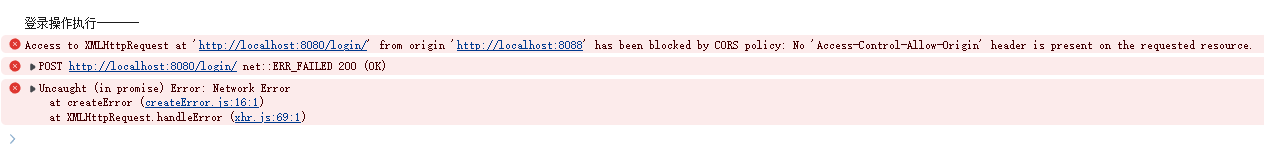
\includegraphics[width=0.9\linewidth]{error.png}
\end{figure}
错误提示表明前端应用(运行在 http://localhost:8088)试图通过 AJAX 请求向后端服务(运行在 http://localhost:8080)发送登录请求,但由于浏览器的跨域安全策略(CORS policy),请求被拒绝了,解决方案:添加 @CrossOrigin(origins = http://localhost:8088)在后端代码中配置 CORS,允许来自 http://localhost:8088 的跨域请求
\begin{lstlisting}
@RestController
public class LoginController
{
    @Autowired
    private LoginServiceImpl loginService;
    @CrossOrigin(origins="http://localhost:8088")
    @PostMapping("/login")
    public ApiResult login(...)
}
\end{minted}
\end{lstlisting}

\section{软件运行效果}
\begin{figure}[H]
    \centering
    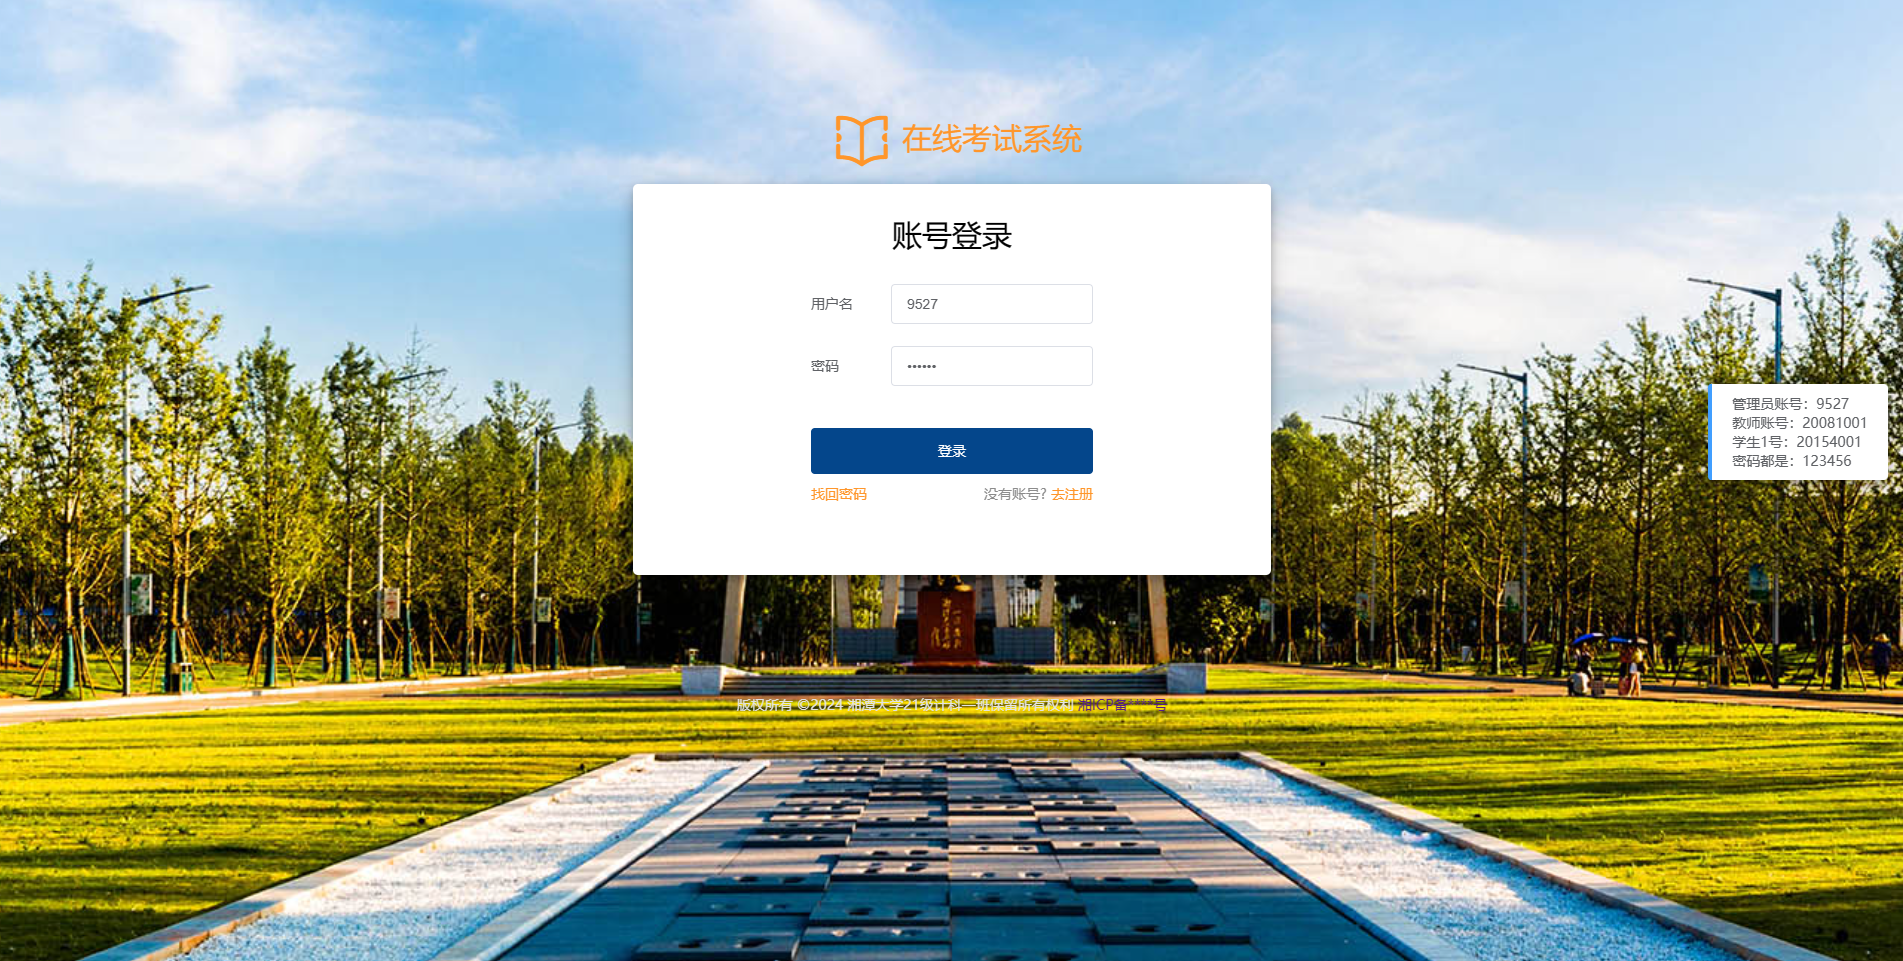
\includegraphics[width=0.8\linewidth]{performance (1).png}
\end{figure}
\begin{figure}[H]
    \centering
    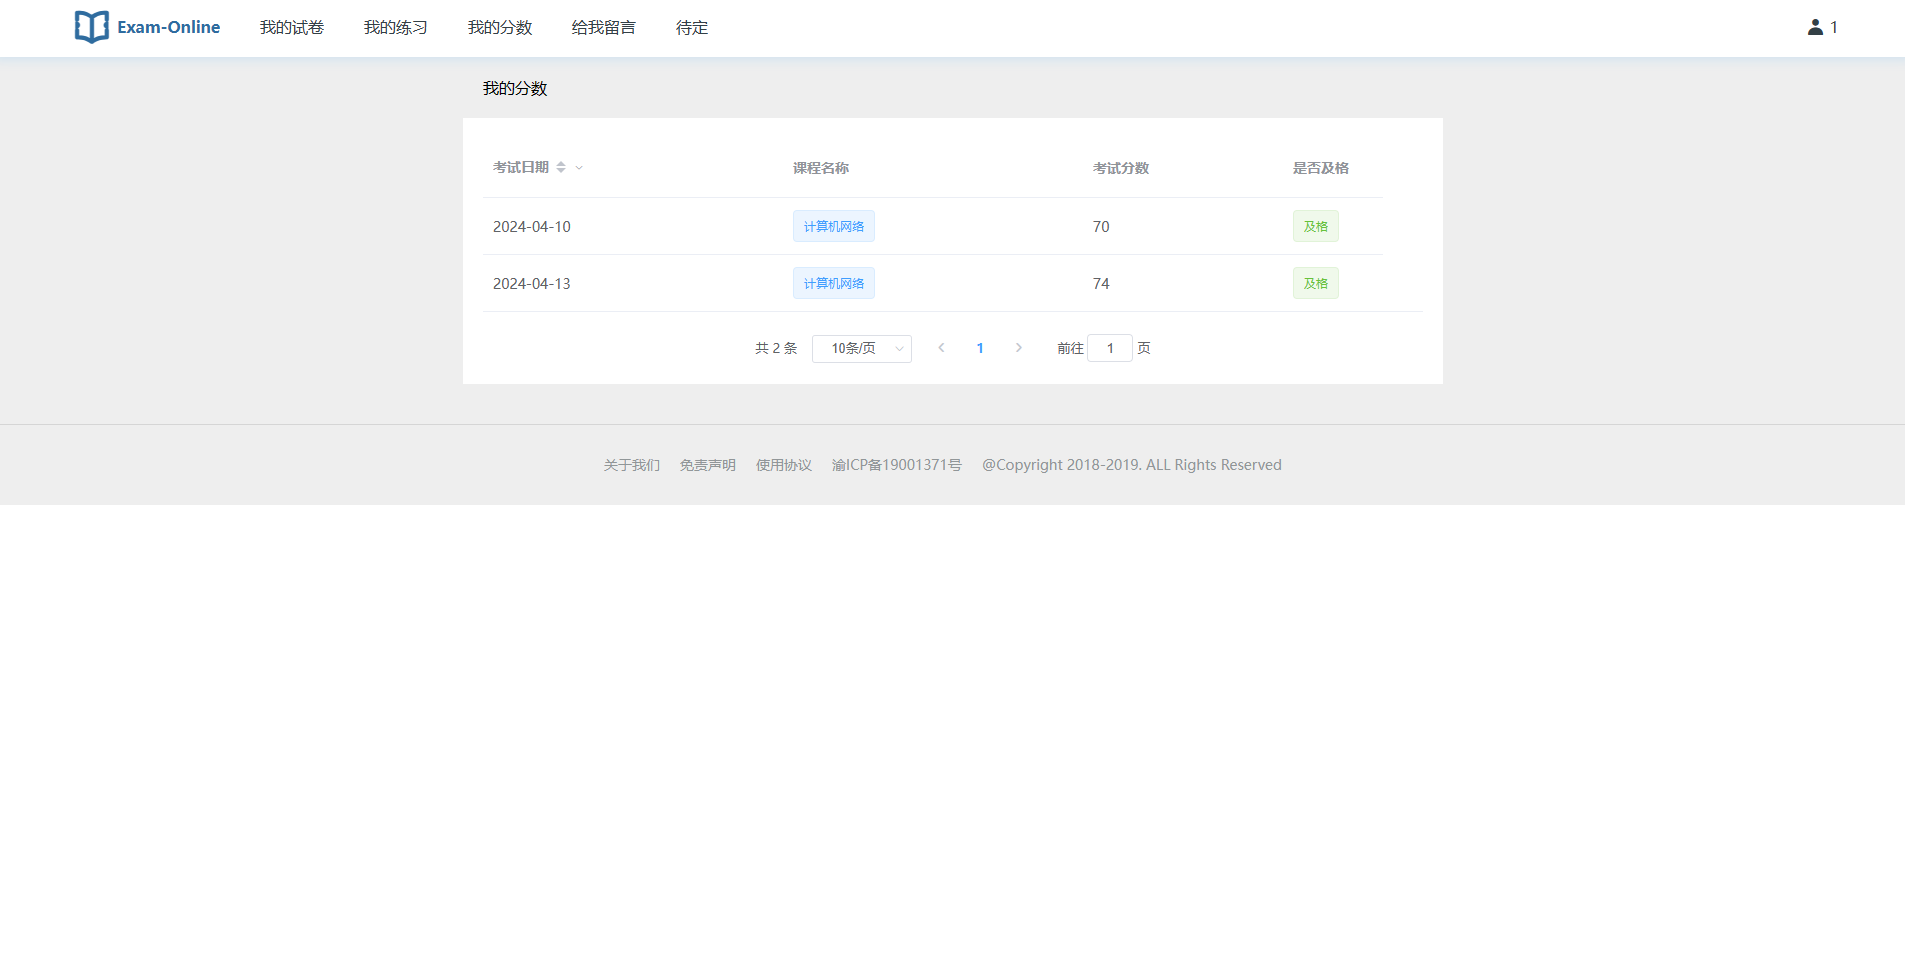
\includegraphics[width=0.8\linewidth]{performance (2).png}
\end{figure}
\begin{figure}[H]
    \centering
    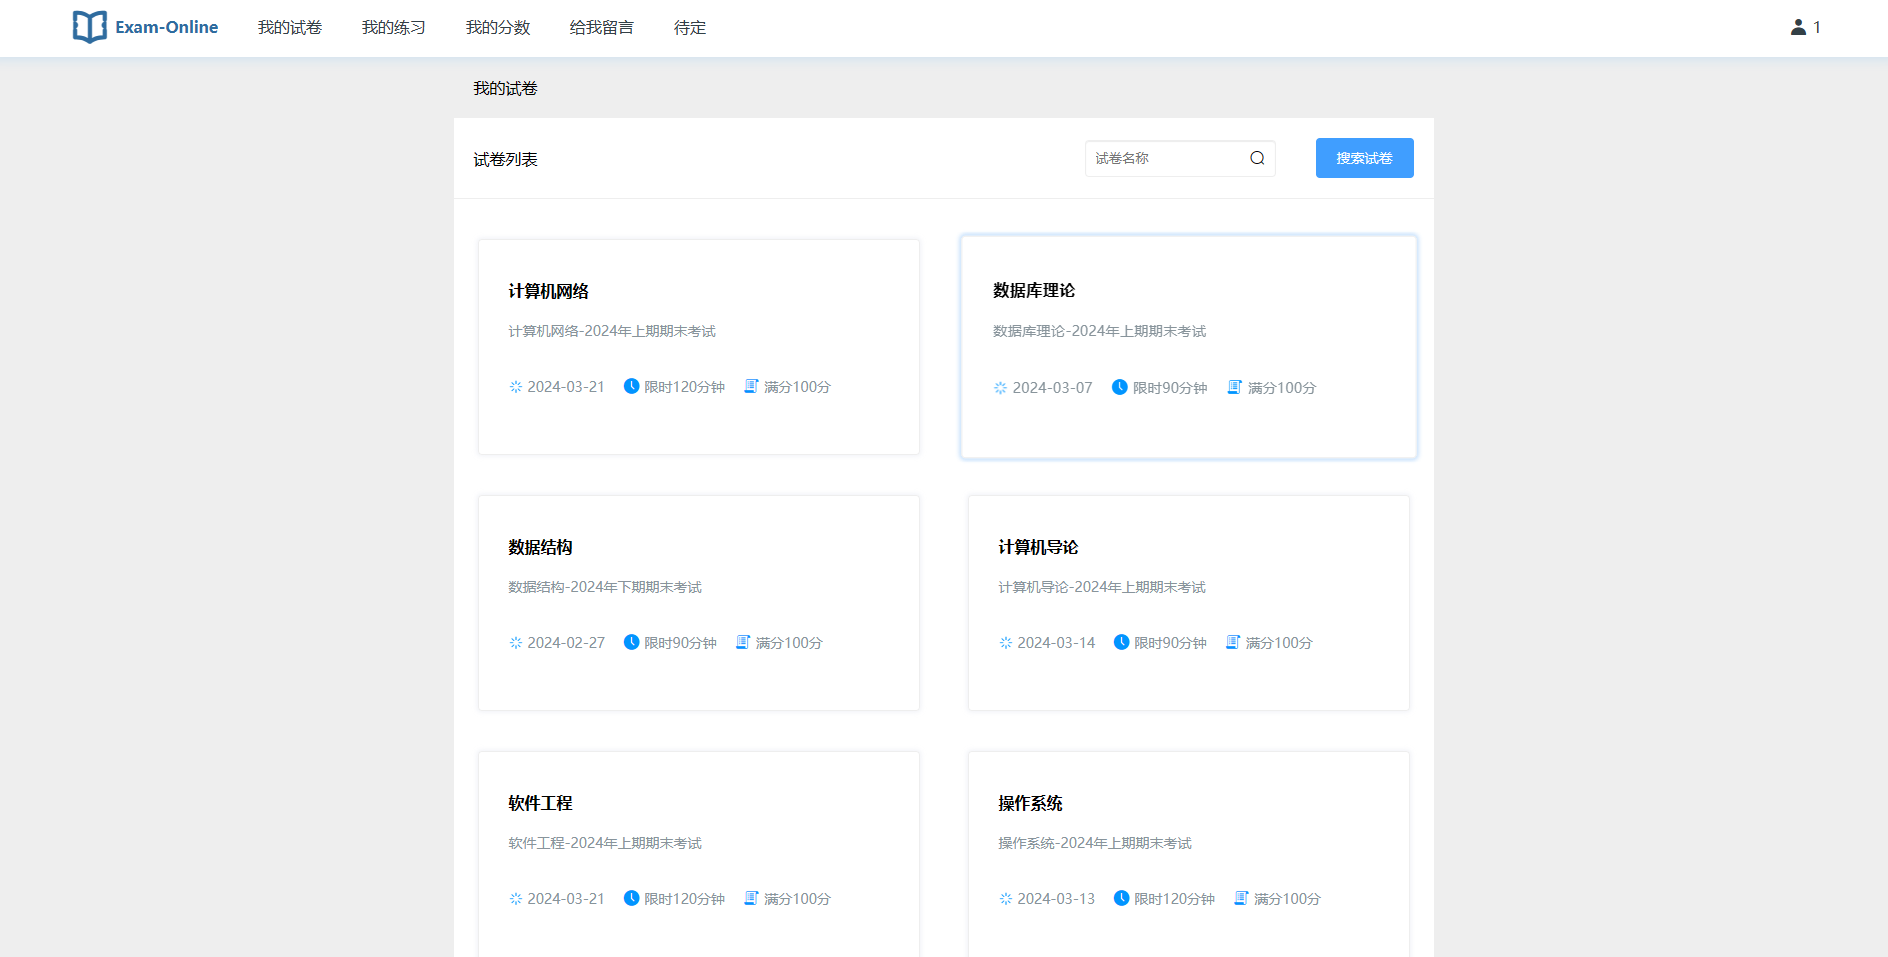
\includegraphics[width=0.8\linewidth]{performance (3).png}
\end{figure}
\begin{figure}[H]
    \centering
    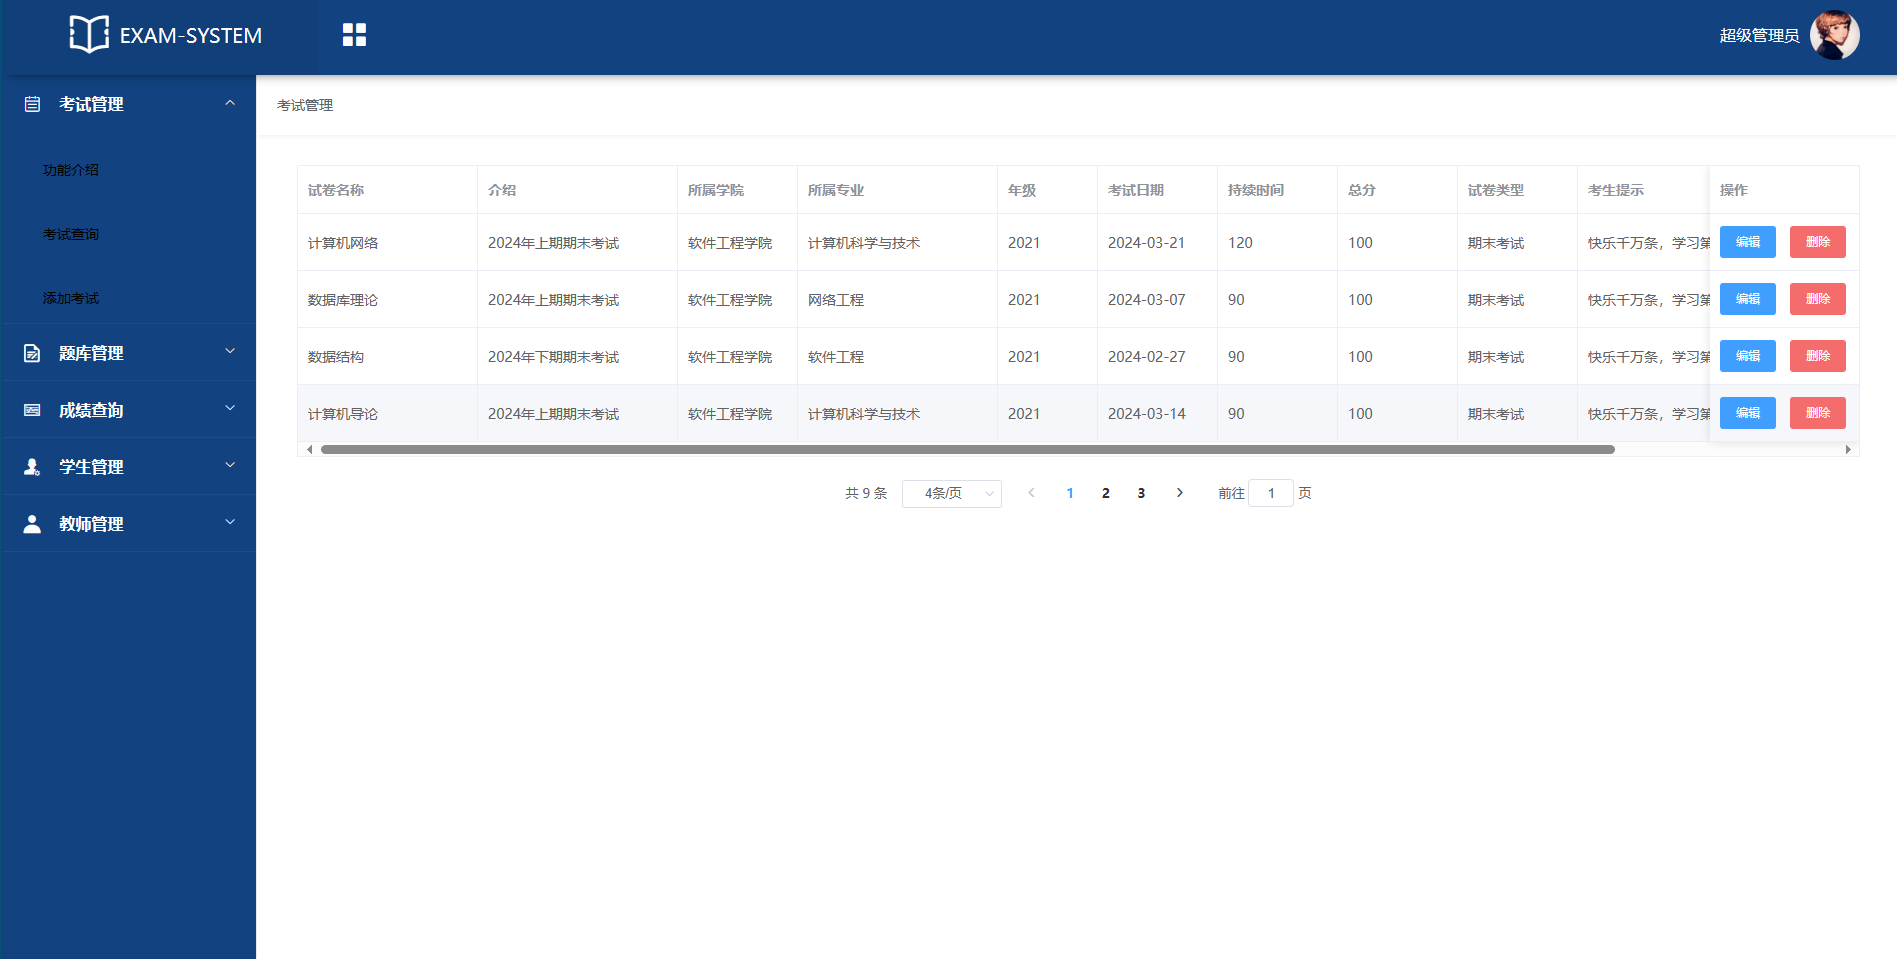
\includegraphics[width=0.8\linewidth]{performance (4).png}
\end{figure}
\begin{figure}[H]
    \centering
    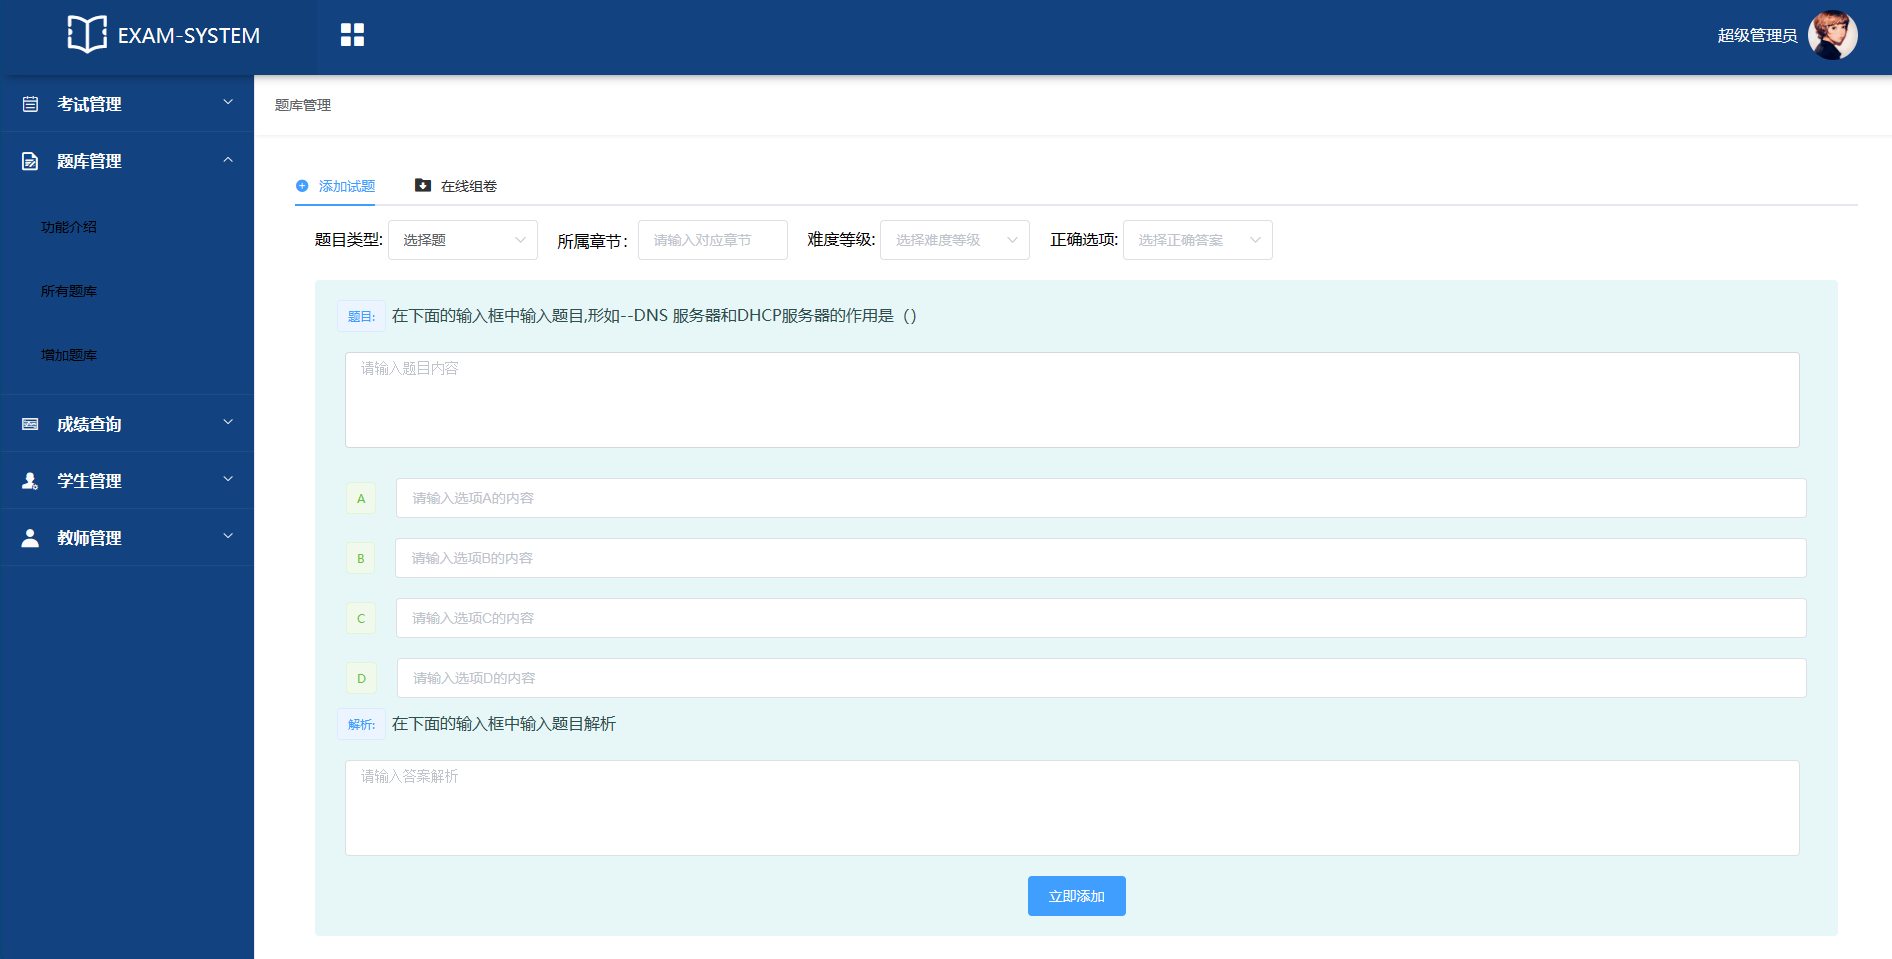
\includegraphics[width=0.8\linewidth]{performance (5).png}
\end{figure}

\section{设计体会}
团队协作开发基于SpringBoot\&Vue的在线考试系统是一次非常有收获的经历。在项目中,我们不仅学习了如何有效整合后端SpringBoot和前端Vue技术,还通过详细的需求分析和系统设计,建立起清晰的开发路线和良好的团队协作模式。每位成员负责不同的模块,通过持续的沟通和协作解决了许多技术难题,同时重视质量保证和测试工作,确保了系统的稳定性和可靠性。这个过程不仅提升了我们的技术能力,还加强了团队的凝聚力和问题解决能力,为未来的项目经验积累和团队合作打下了坚实的基础

\begin{thebibliography}{99}
\bibitem{ref1}Larman C. Applying UML and Patterns: An Introduction to Object-Oriented Analysis and Design and Iterative Development[M]. 2006-5.
\end{thebibliography}


\end{document}
